% This must be in the first 5 lines to tell arXiv to use pdfLaTeX, which is strongly recommended.
\pdfoutput=1
% In particular, the hyperref package requires pdfLaTeX in order to break URLs across lines.

\documentclass[11pt]{article}

% Remove the "review" option to generate the final version.
\usepackage[review]{EMNLP2023}

% Standard package includes
\usepackage{times}
\usepackage{latexsym}
\usepackage{float}
\usepackage{tikz}
\usetikzlibrary{positioning}

% For proper rendering and hyphenation of words containing Latin characters (including in bib files)
\usepackage[T1]{fontenc}
% For Vietnamese characters
% \usepackage[T5]{fontenc}
% See https://www.latex-project.org/help/documentation/encguide.pdf for other character sets

% This assumes your files are encoded as UTF8
\usepackage[utf8]{inputenc}

% This is not strictly necessary and may be commented out.
% However, it will improve the layout of the manuscript,
% and will typically save some space.
\usepackage{microtype}

% This is also not strictly necessary and may be commented out.
% However, it will improve the aesthetics of text in
% the typewriter font.
% \usepackage{inconsolata}

\usepackage{microtype}
\usepackage{enumitem}
\usepackage{times}
\usepackage{latexsym}
\usepackage{xspace}
\usepackage{booktabs}
\usepackage{multirow}
\usepackage{makecell}
\usepackage{color}
\usepackage{microtype}
\usepackage{amsmath}
\usepackage{graphicx}
\usepackage{amssymb,amsthm}
\usepackage{xcolor}
\usepackage{subcaption}
\usepackage{caption}
%\usepackage{paralist}
\usepackage{cleveref}
\usepackage{booktabs}
\usepackage{url}
\usepackage[normalem]{ulem}
\useunder{\uline}{\ul}{}
\newcommand{\todo}[1]{{\color{red}{#1}}}
\newcommand{\our}{\mbox{\textsc{DocSplit}}}
\newcommand{\ourbert}{$\our_{\mathrm{bert}}$}
\newcommand{\ourlong}{$\our_{\mathrm{long}}$}

\newcommand{\fixme}[1]{{\color{red}{FIXME: {#1}}}}
% If the title and author information does not fit in the area allocated, uncomment the following
%
%\setlength\titlebox{<dim>}
%
% and set <dim> to something 5cm or larger.

\title{$\our$: Simple Contrastive Pretraining for \\ Large Document Embeddings}

% Author information can be set in various styles:
% For several authors from the same institution:
% \author{Author 1 \and ... \and Author n \\
%         Address line \\ ... \\ Address line}
% if the names do not fit well on one line use
%         Author 1 \\ {\bf Author 2} \\ ... \\ {\bf Author n} \\
% For authors from different institutions:
% \author{Author 1 \\ Address line \\  ... \\ Address line
%         \And  ... \And
%         Author n \\ Address line \\ ... \\ Address line}
% To start a separate ``row'' of authors use \AND, as in
% \author{Author 1 \\ Address line \\  ... \\ Address line
%         \AND
%         Author 2 \\ Address line \\ ... \\ Address line \And
%         Author 3 \\ Address line \\ ... \\ Address line}

% \author{First Author \\
%   Affiliation / Address line 1 \\
%   Affiliation / Address line 2 \\
%   Affiliation / Address line 3 \\
%   \texttt{email@domain} \\\And
%   Second Author \\
%   Affiliation / Address line 1 \\
%   Affiliation / Address line 2 \\
%   Affiliation / Address line 3 \\
%   \texttt{email@domain} \\}

\author{Yujie Wang \\
  Claremont Graduate University 
  \texttt{yujie.wang@cgu.edu} \\\And
  Mike Izbicki \\
  Claremont McKenna College
  \texttt{Michael.Izbicki@ClaremontMcKenna.edu} \\}

\begin{document}
\maketitle
\begin{abstract}

Existing model pretraining methods only consider local information.
For example, in the popular token masking strategy, the words closer to the masked token are more important for prediction than words far away.
This results in pretrained models that generate high-quality sentence embeddings, but low-quality embeddings for large documents.
We propose a new pretraining method called $\our$ which forces models to consider the entire global context of a large document.
Our method uses a contrastive loss where the positive examples are randomly sampled sections of the input document, and negative examples are randomly sampled sections of unrelated documents.
Like previous pretraining methods, $\our$ is fully unsupervised, easy to implement, and can be used to pretrain any model
architecture.
Our experiments show that $\our$ outperforms other pretraining methods for document classification, few shot learning, and document retrieval tasks.
\end{abstract}



\section{Introduction}

%The standard transformer model 

Generating high-quality text embeddings for documents is a long-standing open problem.
Most previous studies focus on either learning sentence-level representations~\cite{Hill2016LearningDR, Logeswaran2018AnEF, Gao2021SimCSESC} where training data usually contain short text or designing specific model structures for larger-range dependencies~\cite{Beltagy2020LongformerTL, Zaheer2020BigBT},
but effective and efficient document representation learning methods are less explored.

\begin{figure}
    \centering
    %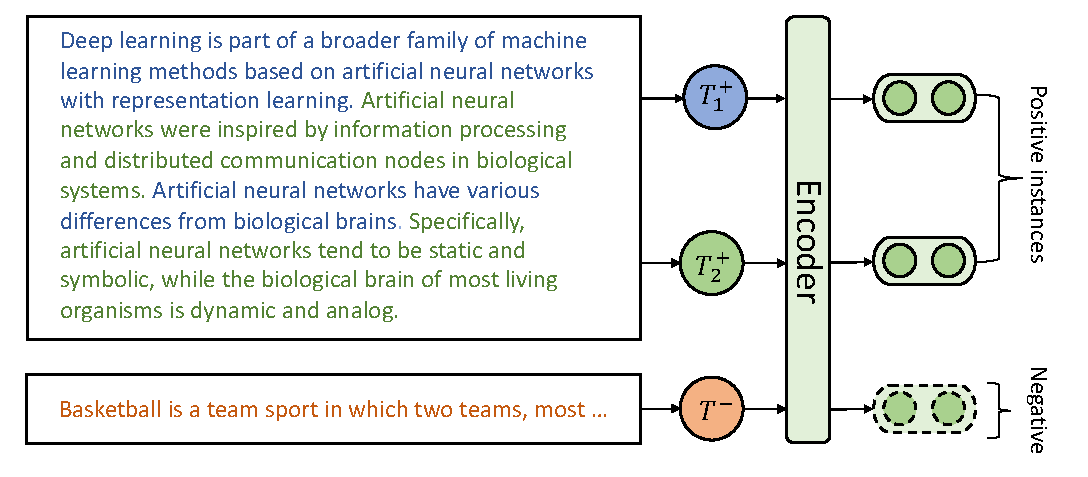
\includegraphics[width=\columnwidth]{fig/docsplit.pdf}
    %\includegraphics[width=\columnwidth]{example-image-golden.pdf}
    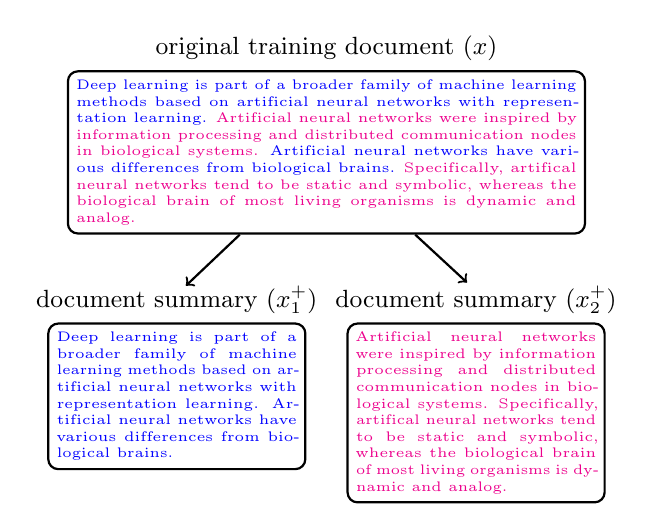
\begin{tikzpicture}
\small
    \node[draw,thick,rounded corners=.05in] (doc) [label=above:original training document ($x$)]{
\tiny
    \parbox{2.5in}{
    \color{blue}
    Deep learning is part of a broader family  of machine learning methods based on artificial neural networks with representation learning.
    \color{magenta}
    Artificial neural networks were inspired by information processing and distributed communication nodes in biological systems.
    \color{blue}
    Artificial neural networks have various differences from biological brains.
    \color{magenta}
    Specifically, artifical neural networks tend to be static and symbolic, whereas the biological brain of most living organisms is dynamic and analog.
    }
};
\node[below=of doc,node distance=0.0in] (placeholder) {};
    \node[draw,thick,rounded corners=.05in,left of=placeholder,node distance=0.1in,anchor=north east]  (x1) [label=above:document summary ($x_1^+$)] {
    \tiny
    \color{blue}
    \parbox{1.2in}{
    Deep learning is part of a broader family  of machine learning methods based on artificial neural networks with representation learning.
    Artificial neural networks have various differences from biological brains.
}};
    \node[draw,thick,rounded corners=.05in,right of=placeholder,node distance=0.1in, anchor=north west] (x2) [label=above:document summary ($x_2^+$)]{
    \tiny
    \color{magenta}
    \parbox{1.2in}{
    Artificial neural networks were inspired by information processing and distributed communication nodes in biological systems.
    Specifically, artifical neural networks tend to be static and symbolic, whereas the biological brain of most living organisms is dynamic and analog.
}
};

    \node[above of=x1, node distance=0.51in] (x1a) {};
    \node[above of=x2, node distance=0.61in] (x2a) {};
    \draw[->,thick] (doc) -- (x1a);
    \draw[->,thick] (doc) -- (x2a);
\end{tikzpicture}

\caption{
    In $\our$ pretraining,
    an input document ($x$) is split into two new document summaries ($x_1^+$ and $x_2^+$) by randomly assigning each sentence to one of the new summaries.
    These new summaries are then used as positive instances for contrastive learning,
    which forces the model to represent these summaries with similar embeddings.
    %$\our$ is a new pretraining strategy that uses contrastive learning.
    %The hard part of contrastive learning is generating positive instances.
    %$\our$ generates these pairs from an input data point by randomly assigning each sentence in the input document to one of the pairs.
    %For each sentence in the input document, the sentence is randomly assigned to one of the positive instances ({\color{blue}{$T_1^+$} or \color{green}{$T_2^+$}).
    %Overall framework of \our. The document is randomly divided into two exclusive subsets of sentences and the two subsets work as positive pairs for contrastive learning. Other instances in the same batch are used as negatives.
}
\label{overall}
\end{figure}

This paper presents $\our$, the first unsupervised pretraining method designed specifically for large documents.
$\our$ is simple to use,
and it can be applied to any model architecture to improve document representations. 
$\our$ uses contrastive learning,
and our key contribution is a new method for generating positive samples for contrastive learning.
Figure \ref{overall} provides a graphical illustration of the method,
and Section \ref{sec:method} describes the implementation details and intuition.

Section \ref{sec:related} describes how $\our$ improves prior work.
We begin by demonstrating that prior work on contrastive pretraining has focused only on sentence-level representations.
Then we show that work on model architectures designed for large documents has ignored the problem of better pretraining methods designed to work with these architectures.

%Our paper is organized as follows.
%Section \ref{sec:method} formally describes the $\our$ pretraining method.
%Section \ref{sec:related} describes t
%We highlight how our $\our$ method improves on related contrastive learning frameworks like \texttt{SimCSE}

In Section \ref{sec:experiments}, we describe two pretrained models based on the BERT architecture (for fair comparison to other contrastive losses) and the LongFormer architecture (for optimal performance on large documents).
We evaluate these models on standard large document classification, few shot learning, and document retrieval tasks.
We find that models pretrained using $\our$ significantly outperform models pretrained with all other published methods.

%We conclude in Section~\ref{sec:conclusion} by emphasizing that all of our models and datasets are open source.

%To this end, we first investigate the information redundancy with two methods (details in Appendix~\ref{app:redundacy}) on five datasets for different lengths of documents.
%We find (1) information redundancy is larger as the length of the documents is increasing and (2) sentences from the same document usually contain repeated information. 
%Based on this observation, we can assume that the model can still learn the semantics of documents even if we drop some sentences. Hence, as shown in Figure~\ref{overall}, we randomly divide the original documents into two parts by sentences as positive pairs. Due to redundancies, our model can still recognize the two pairs have the same semantics. 
%The intuition behind this method is that we expect the model will pull representations of two subsets together in the latent space by paying more attention to common keywords so that the model can learn key information from documents automatically. 

%To evaluate the quality of document embeddings, we conduct standard and few-shot text classification on five large document datasets involved in News and scientific articles. Moreover, to further validate the effectiveness of our method, we also conduct document retrieval on the AAN dataset which is designed for long document understanding evaluation.
%The experimental results show that \our~with two kinds of model structures (i.e.,~BERT and Longformer) can both achieve significant improvements compared to state-of-the-art baselines.

% The recurrent connections in models like the LSTM~\cite{Hochreiter1997LongSM} and GRU~\cite{Cho2014OnTP} allow information at all locations in the document to influence the final embedding,
% but they are slow to train because the models must consider each word sequentially.
% The Transformer architecture~\cite{Vaswani2017AttentionIA} uses self-attention with no recurrent connections,
% and so can be trained much faster than recurrent models.
% This has led to the widespread use of language models like BERT~\cite{Devlin2019BERTPO} and ELMO~\cite{Peters2018DeepCW} that are pre-trained on large scale web data.
% Unfortunately, the memory requirements of self-attention scale as $O(n^2)$ and so are not suitable for long documents.
%Large scale pre-trained transformers like BERT~\cite{} and ELMO~\cite{} are currently state-of-the-art for many NLP tasks that require only short-term dependencies in text.
%These transformers do not handle long-term dependencies well, however, because they require $O(n^2)$ memory for the size of the context window.
% The LongFormer~\cite{Beltagy2020LongformerTL} and BigBird~\cite{Zaheer2020BigBT} models allow larger-range dependencies by introducing improved attention mechanisms that reduce the memory requirements down to $O(n)$.
% This previous research focuses on designing new model architectures suitable for long text,
% but in this paper we present the $\our$ training procedure that can work with any model architecture.
%All of this previous research focuses on designing new model architectures.
%Our paper introduces a new training method called the $\our$ that works for any model architecture.



% $\our$ is the first unsupervised training method designed specifically for long text.
% Previous methods for training on long text either require supervision~\cite{} or use the masked language modeling (MLM) technique~\cite{}.
% In MLM, we replace a token from the input text with a special ``mask'' token and train the model to predict which token was removed.
% The MLM pretraining method has been shown to work well for short-text documents~\cite{},
% but we argue that it sub-optimal for long text because most of the information for predicting the masked token is available near the token.
% The $\our$ pretraining technique is designed to force the model to learn long range dependencies within a document.
% Specifically, $\our$ uses contranstive learning,
% and our key contribution is a new method for generating the positive samples for contrastive learning (see Figure~\ref{overall} above).
%The most similar work to our own is the \texttt{SimCSE} method which uses contrastive learning to pre-train text models,

%Supervised methods cannot be used for large-scale pretraining of models, however, so we present the 

\section{Method}

\label{sec:method}
We first review contrastive learning at a high level, then we describe our \our~method.

%\subsection{Overview of Contrastive Learning}
%
%Contrastive learning is a method for unsupervised pretraining of deep neural networks.
%The idea was first introduced by \citet{Hadsell2006DimensionalityRB},
%but saw a resurgence in popularity when it was used to pretrain multi-purpose vision models \cite{Chen2020ASF}.
%It then became widely used in the natural language processing community to generate state-of-the-art pretrained models.
%
%%The original BERT transformer architecture \citep{Devlin2019BERTPO} was pretrained with token masking.
%In this section we provide an intuitive, non-mathematical overview of contrastive learning.
%Contrastive learning is a 

\subsection{Contrastive Learning}
Contrastive Learning learns effective representations by pulling semantically close neighbors together and pushing apart non-neighbors in the latent space~\cite{Hadsell2006DimensionalityRB}.
Each data point $x$ is converted into a contrastive instance $\{x^{+}_1, x^{+}_2, x_1^{-},\dots,x_{N}^{-}\}$ that includes two positive examples and $N$ negative examples.
Intuitively, the positive instances should be semantically similar to each other (they will be pushed together) and the negative instances should be semantically dissimilar to the positive instances (they will be pushed away).
%and their representations $\{\mathbf{h}, \mathbf{h}^{+}, \mathbf{h}_1^{-}, \dots,
%\mathbf{h}_{N-1}^{-}\}$, where $x$ and $x^{+}$ are semantically related.
Following recent influential work \cite{Chen2020ASF,Gao2021SimCSESC,Li2022UCTopicUC}, we use cross entropy as our loss function.
As the mathematical details are technical and not relevant to our discussion,
we do not reproduce them here.
%We follow the contrastive learning framework~~\cite{Chen2020ASF, Li2022UCTopicUC} and take cross-entropy as our objective function:
%\begin{equation}
%\label{cl}
    %l = -\log \frac{e^{\mathrm{sim}(\mathbf{h}, \mathbf{h}^{+})/\tau}}{e^{\mathrm{sim}(\mathbf{h}, \mathbf{h}^{+})/\tau}+ \sum_{i=1}^{N-1}e^{\mathrm{sim}(\mathbf{h}, \mathbf{h}_i^{-})/\tau}}
%\end{equation}
%where $\tau$ is a temperature hyperparameter and $\mathrm{sim}(\mathbf{h}_1, \mathbf{h}_2)$ is the cosine similarity $\frac{\mathbf{h}_1^{\top}\mathbf{h}_2}{\Vert \mathbf{h}_1 \Vert \cdot \Vert \mathbf{h}_2 \Vert}$.
%
%In this work, we encode input texts using a pre-trained language model such as BERT~\cite{Devlin2019BERTPO}. Following BERT, we use the first special token \texttt{[CLS]} as the representation of the input and fine-tune all the parameters using the contrastive learning objective in Equation~\ref{cl}.

There are many model training methods that use contrastive learning, and what differentiates these methods is how they convert the data point $x$ into the contrastive instance.
%For our purposes, the important part of contrastive learning is how to convert the data point $x$ into the contrastive instance of positive and negative pairs.
It is standard practice to use in-batch instances for the negative pairs,
and so all that remains is designing a method for constructing the positive pairs $(x_1^+, x_2^+)$.
%For negative instances, we use in-batch instances following previous contrastive frameworks~\cite{Gao2021SimCSESC, Li2022UCTopicUC}.
%The critical problem in contrastive learning is how to construct positive pairs $(x, x^{+})$.
%In representation learning for visual tasks~\cite{Chen2020ASF}, an effective solution is to take two random transformations of the same image (e.g.,~flipping, rotation).
%Similarly, in language representations, previous works~\cite{Gao2021SimCSESC, Karpukhin2020DensePR, Meng2021COCOLMCA, Li2022UCTopicUC} apply augmentation techniques such as dropout, word deletion, reordering, and masking.

\subsection{Document Splitting ($\our$)}
Our main contribution is the $\our$ method to construct the positive pairs needed for contrastive learning.
The idea is simple to describe and implement.
Given an input document, we first split the document into sentences.
Then each sentence is randomly assigned to either the $x^+_1$ or $x^+_2$ document.

This splitting procedure results in two documents that can be thought of as ``summaries'' of the original document.
These summaries will have similar semantic content,
and the contrastive loss will ensure that these two documents have similar embeddings.
Notice that because there is randomness in the document splitting procedure,
multiple passes over the same data points will result in different contrastive instance pairs being generated.
This provides built-in overfitting resistance through data augmentation when multiple epochs of the training data are used.

%There are several intuitive reasons why we should expect $\our$
%~to generate good document pairs.
%First, we can think of each positive instance as a summary of the original document.
%Second, our splitting strategy captures global information about the document.

%The basic idea of positive instance construction for contrastive learning is adding random noises to the original data for augmentation. 
%The augmented data should have similar representations to the original data. 
%Models trained by contrastive losses on augmented data will have an increased ability to learn important features in the data.
%To add random noises in documents, we find documents usually has higher information redundancy than sentences (Table~\ref{redundancy} in Appendix). 
%With this observation, we can have an assumption: 
%the semantics of a document will not be changed even if we drop half of the document. 
%We can construct positive pairs under this assumption easily on any text dataset without supervision.
%Specifically, for each document in the dataset, we randomly split sentences in the document into two subsets and the two sentence sets do not have intersections. 
%In the two subsets, we keep the order of sentences in the original document to form two new documents. 
%According to our assumption, the two new documents should have the same semantics and hence they are used as a positive pair in contrastive learning. 
%
%Consider an example (in Figure~\ref{overall}) to understand our positive instance construction process:
%Suppose we have a document $T = (s_1, s_2,\dots,s_n)$ where $s_i$ is the $i$-th sentence in document and $n$ is the number of sentences, each sentence will be sent to anchor set or positive set with the same probability ($50\%$). 
%The sentences in the same set (i.e.,~anchor or positive) will be concatenated in the same order of $T$ to form one positive pair $(T^+_1, T^+_2)$ for contrastive learning. 
%Positive pairs constructed by this method will not contain the same sentence and hence prevent models from overfitting on recognizing the same sentences. 
%Instead, models are guided to learn keywords appearing in positive instances so as to improve the ability to recognize key information. 
%We split the document at sentence level instead of word level (e.g.,~word deletion for augmentation) because the word-level splitting will cause the discrepancy between pretraining and finetuning and then lead to performance decay.

\section{Related Work}
\label{sec:related}

There are two categories of related work:
models trained using contrastive learning,
and models designed for large documents.

\subsection{Contrastive Pretraining}
\label{sec:contrastive}

Contrastive learning has shown remarkable recent success for developing sentence embeddings.
The simplest method is SimCSE \cite{Gao2021SimCSESC},
which uses dropout to generate correlated positive samples.
The contrastive tension method \cite{Carlsson2021SemanticRW} is similarly generic,
but has a much more complicated implementation involving multiple models trained jointly.
Because both of these pretraining strategies are generic,
they can be used with any type of input including documents;
but they do not take explicit advantage of document structure.
%CT-BERT \cite{Carlsson2021SemanticRW} uses a pair of training models (contrastive tension).
The INSTRUCTOR model \cite{Su2022OneEA} is the current state-of-the-art model for most downstream tasks.
The contrastive objective for this model requires a specially constructed corpus of manual-human annotations,
and this corpus is limited only to sentence-level annotations instead of document-level annotations.
We show that our model significantly improves on INSTRUCTOR on document level tasks, and it is not clear how to extend the INSTRUCTOR model to document-level tasks because human annotation for documents is significantly more expensive than for sentences.

The Contriever model \cite{Izacard2021UnsupervisedDI} uses a contrastive objective most similar to our own.
They use the document cropping and inverse cloze tasks for pretraining.
In document cropping, a document is divided in half and the two halves are used as the positive samples;
in inverse cloze, a contiguous substring of the document is used as one positive sample and all other strings are used as the negative sample.
The $\our$ pretraining method can be seen as a generalization of these methods.
%It is evaluated only on information retrieval setting.
%INSTRUCTOR~\cite{Su2022OneEA} uses instruction tuning.
%They create a manually annotated corpus of 330 different datasets.

\subsection{Large Document Architectures}

%In order to demonstrate that $\our$ is widely applicable,
%we pretrain two models using two different architectures.

All of the models discussed in Section \ref{sec:contrastive} above are based off of the BERT architecture \cite{Devlin2019BERTPO}.
This architecture uses an attention mechanism that requires $O(n^2)$ memory and runtime,
where $n$ is the size of the attention window.
The maximum size of a document that a model can understand is limited by this window size,
and so compute for these models scales quadratically with the length of the documents.

A growing body of research focuses on developing new architectures with reduced computational requirements that enable processing larger documents.
The LongFormer \cite{Beltagy2020LongformerTL} and BigBird \cite{Zaheer2020BigBT} models pioneered this line of research,
and both models reduce the runtime of the attention mechanism to $O(n)$.
%A variety of other architectures have subsequently been proposed like the Informer \cite{zhou2021informer}, Switch Transformer \cite{fedus2022switch}, Performer \cite{choromanski2020rethinking}, and LinFormer \cite{wang2020linformer}
A variety of other architectures have subsequently been proposed \cite[e.g.][]{zhou2021informer,fedus2022switch,choromanski2020rethinking,wang2020linformer,liu2022ecoformer}.
\citet{tay2022efficient} provide a survey of this large body of work.
Importantly, all of this research focuses only on improving the computational aspects of model architecture,
and none of these models use a training objective designed specifically for large documents.
Because the $\our$~pretraining method is model agnostic,
we can easily apply it to any of these newly proposed model architectures.
For computational reasons, we limit our experimental comparisons in Section \ref{sec:experiments} below to the LongFormer and BigBird models since these are the two most influential model architectures designed for large documents.
We find a large performance improvement when these models are trained with $\our$,
and expect this performance improvement would extend to similar models as well.

%We call the second model \ourlong~because it is pretrained on the LongFormer architecture \cite{Beltagy2020LongformerTL}.
%LongFormer uses a modified attention head that requires only $O(n)$ compute instead of the standard $O(n^2)$ that Bert uses,
%and so can handle larger context windows needed for large documents.
%Our \ourlong pretrained model inherits this computational advantage.
%We also compare to the BigBird~\cite{Zaheer2020BigBT} model,
%which is architecturally similar.


\section{Experiments}

\label{sec:experiments}

%To properly evaluate our $\our$~pretraining method against the related work described in Section \ref{sec:related} above,
%we pretrain two different models.
%The first model \ourbert~uses the same BERT architecture that all other contrastive models of Section \ref{sec:contrastive} were trained on.
%The second model \ourlong~uses the LongFormer architecture.

We perform a careful ablation study to isolate the effects of the $\our$ pretraining method on downstream task performance.
First, we pretrain separate models for each group of baseline models described in Section \ref{sec:related} above.
%In particular, the \ourbert~model is trained on the BERT architecture and allows us to directly compare the performance of all contrastively pretrained models of \ref{sec:contrastive}.
%\footnote{We do not compare to the popular RoBERTa~\cite{Liu2019RoBERTaAR}, IS-BERT~\cite{Zhang2020AnUS} and GTR~\cite{Ni2021LargeDE} models because SimCSE and INSTRUCTOR achieve better results than these methods according to their papers.}
%The \ourlong~model is trained on the LongFormer architecture and allows to see how better pretraining drastically improves the performance of these architectures designed specifically for large documents.
Then, we perform downstream experiments on standard classification, few-shot learning, and document retrieval tasks.
In all cases, our pretrained models significantly outperform prior work.


%We first describe how we pretrain our model.
%Then we describe our classification, few-shot learning, and information retrieval evaluation tasks.

%We use a standard experimental setup to evaluate the effectiveness of \our.
%First, we pretr
%
%We evaluate the effectiveness of \our~using a standard procedureby pretraining two models on English language wikipedia.
%Then we finetune the model
%
%In this section, we evaluate the effectiveness of our method by conducting text classification tasks. 
%To eliminate the influence of different model structures and focus on the quality of text embeddings. 
%We freeze the parameters of different text encoders and fine-tune only a multi-layer perceptron (MLP) to classify the embeddings of text encoders.
%We also visualize the attention weights between baselines and \our.
%
%We do not use semantic textual similarity (STS) tasks~\cite{Agirre2012SemEval2012T6} because the sentences in these tasks are short which is not suitable to evaluate large document embeddings.
\begin{table*}
    \centering
% \scalebox{0.7}{
% \setlength{\tabcolsep}{1.mm}{
    %\begin{tabular}{@{}lR{0.75in}R{0.75in}R{0.75in}R{0.75in}R{0.75in}R{0.75in}@{}}
\small
\begin{tabular}{l|cccccccccc}
\toprule
 Datasets   & \multicolumn{2}{c}{FakeNews}     & \multicolumn{2}{c}{20News}         &\multicolumn{2}{c}{arXiv}     &\multicolumn{2}{c}{NYT}        & \multicolumn{2}{c}{BBCNews} \\
 \cmidrule(l){1-1} 
\cmidrule(l){2-3} 
\cmidrule(l){4-5}
\cmidrule(l){6-7}
\cmidrule(l){8-9}
\cmidrule(l){10-11}
Metrics    & Acc & F1   & Acc & F1    & Acc & F1    & Acc & F1      & Acc & F1 \\

\midrule
BERT      &54.98  &42.17    &62.34  &54.19    &68.52  &20.46     &95.11  &92.65      &91.06  &90.34 \\
CT-BERT       &55.19  &42.53    &65.76  &63.37  &71.61 &26.09  &95.69  &91.59  &90.32  &88.87   \\
SimCSE &58.48  &47.46    &74.02  &72.57    &74.46  &30.01     &97.17  &94.69      &94.12  &93.86  \\
SimCSE$_{\mathrm{long}}$ &58.37  &47.56    &73.51  &72.05    &73.16 &29.41  &97.25 &93.83   &94.22  &94.30 \\
Contriever   &58.21 &47.25   &75.86 &74.28 &75.35 &28.24 &96.94 &92.71 &94.66 &94.57            \\
INSTRUCTOR  &59.26 &47.92  & --
& -- &75.52 &30.46 &97.06 &93.66 &95.19 &95.16 \\
    \ourbert        &\textbf{60.04}  & \textbf{50.14}   & \textbf{76.89}  &\textbf{74.85}   &\textbf{76.66}  &\textbf{32.24}     &\textbf{98.20}  &\textbf{96.05}      &\textbf{95.56}  &\textbf{95.58}  \\
\midrule
LongFormer  &65.72  &57.66    &73.69  &72.47    &71.66  &25.92     &94.36  &88.39      &96.33  &94.75  \\
BigBird      &57.44  &47.87    &70.35  &68.91    &71.58 &25.05  &97.13 &94.33   &94.11  &94.62 \\
\ourlong  &\textbf{71.60}   &\textbf{61.66}     &\textbf{75.44}  &\textbf{74.38}    &\textbf{77.68}  &\textbf{33.26}     &\textbf{97.90}  &\textbf{95.43}  &\textbf{96.67}  &\textbf{95.91}  \\


\bottomrule
\end{tabular}


    % }}
    \caption{
        In the text classification of Experiment 1, models pretrained with $\our$ outperform baseline models in all cases.
        Larger numbers are better.
    }
    \vspace{-3mm}
    \label{results}
\end{table*}

\subsection{Pretraining Details}

We pretrain two models on two different architectures.
All prior work using contrastive learning discussed in Section \ref{sec:contrastive} above evaluates their pretraining methods on the BERT architecture.
To fairly compare against these methods, we pretrain our \ourbert~model also on this architecture.
Ultimately, however, we are interested in large document performance, and so we expect that a model architecture designed specifically for large documents will improve performance.
We therefore also pretrain the \ourlong~model on the LongFormer architecture.
This second model will be used to evaluate against other models designed specifically for large documents.

To pretrain both models, we follow the standard pretraining procedure for contrastive losses established by \citet{Gao2021SimCSESC} and \citet{Li2022UCTopicUC}.
We simultaneously optimize both the masked language model (MLM) loss (with weight$=0.1$) and the contrastive loss (with temperature $\tau=0.05$).
We use English Wikipedia articles as our pretraining dataset.
These articles are long, and so we expect that a pretraining procedure designed for large documents will improve performance.
The total number of training instances is 6,218,825.
We use AdamW \cite{Kingma2014AdamAM} with a learning rate of 5e-5.
\ourbert uses a batch size of 36.
And due to the larger memory requirements of the LongFormer architecture,
\ourlong uses a batchsize of 12.
For both models, we know that performance improvements on downstream tasks must be due to the pretraining procedure and not the dataset because all baseline models include English language wikipedia in their training set.

%\subsection{Baselines}
%
%We compare our two pre-trained model to baselines with similar architectures and different pretraining strategies.
%
%
%For \ourbert
%(1) Language models trained for general language understanding and sentence embeddings include BERT~\cite{Devlin2019BERTPO}, SimCSE~\cite{Gao2021SimCSESC}~\footnote{SimCSE can be viewed as an ablation model without document splitting.}, CT-BERT~\cite{Carlsson2021SemanticRW}, Contriever~\cite{Izacard2021UnsupervisedDI} and INSTRUCTOR~\cite{Su2022OneEA}. 
%For a fair comparison, we also train a SimCSE with our pretraining dataset (SimCSE$_\mathrm{long}$).
%(2) Transformers specified for long sequences include Longformer~\cite{Beltagy2020LongformerTL} and BigBird~\cite{Zaheer2020BigBT}.
%We train two versions of \our~with BERT and Longformer (i.e.,~\our$_\mathrm{bert}$ and \our$_{\mathrm{long}}$) for comparison.


\subsection{Experiment 1: Text Classification}
%In the standard text classification task, we classify text embeddings with the full training set. 
%Training details are in Appendix~\ref{app:details}.
%
%\textbf{Datasets.}
We fine tune \ourbert, \ourlong, and all baseline models on five standard document datasets.
The datasets are summarized in the table below:%
\footnote{Citations for the datasets are:
Fake News Corpus \url{https://github.com/several27/FakeNewsCorpus};
arXiv articles dataset~\url{https://www.kaggle.com/datasets/Cornell-University/arxiv};
20NewsGroups~\cite{Lang1995NewsWeederLT};
New York Times Annotated Corpus (NYT) ~\cite{sandhaus2008new}; and
BBCNews~\url{http://mlg.ucd.ie/datasets/bbc.html}.
}

\begin{table}[H]
\centering
{
\small
\begin{tabular}{lrrrrrrrr}
\toprule
Dataset & Num Docs & Classes & \multicolumn{2}{c}{Words~/~Doc} &99th &95th &90th &75th \\
    \cmidrule{4-5}
& & & Mean&  Max \\
\midrule
FakeNews &8,558,957 &15 &467 &33,936 &2,949 &1,403 &1,024 &608 \\
arXiv &2,162,833 &38 &138 &925 &289 &255 &230 &181 \\
20News &18,846 &20 &258 &11,554 &1,865 &714 &468 &264\\
NYT &13,081 &5 &650 &5503 &1,264 &1,043 &966 &831\\
BBCNews &2,225 &5 &133 &445 &311 &234 &206 &167\\
\bottomrule
\end{tabular}
}

\label{dataset}
\end{table}

\noindent
%Notice in particular that every dataset has documents that exceed the standard context window length of the BERT model.
%For these documents, we follow the standard procedure and truncate the documents before passing them to BERT-based models.

%\textbf{Results.}
Table~\ref{results} shows the accuracy and F1 score of every model on these datasets.
Notice that \ourbert~out performs all BERT-based models discussed in Section \ref{sec:contrastive},
and \ourlong~outperforms all models on every dataset.
There are no results for INSTRUCTOR on the 20News dataset because INSTRUCTOR was pretrained on 20News,
and the authors state that evaluating INSTRUCTOR on datasets it was pretrained is incorrect due to data contamination.
%Overall, we can see that \our~achieves the best performance over the 4 document datasets (except INSTRUCTOR on 20News due to its data leakage) and consistently improves the document embeddings with BERT and Longformer structures. 
%INSTRUCTOR~\cite{Su2022OneEA} includes 20News in their pretraining datasets which causes data leakage in our experiments, hence INSTRUCTOR results on 20News are not comparable to others.
%Specifically, methods pretrained with contrastive objectives (i.e.,~CT-BERT, SimCSE, Contriever and INSTRUCTOR) outperform general language representations (i.e., BERT and LongFormer) which indicates contrastive objectives designed for text embeddings can largely improve the ability of language models to produce high-quality text embeddings. 
%SimCSE pretrained with our document data (i.e.,~SimCSE$_{\mathrm{long}}$) has similar results as the original SimCSE which indicates simply increasing the length of pretraining text cannot improve document embeddings.
%Under the same model structures, our model achieves $3.9\%$ and $9.4\%$ average macro-F1 improvements with BERT and Longformer structures respectively compared to SimCSE and Longformer. 
%Compared to the state-of-the-art model INSTRUCTOR, our model (\our$_{\mathrm{bert}}$) can achieve $3.4\%$ improvements.
%Hence, our contrastive learning method is effective for document embeddings.


\subsection{Experiment 2: Few-shot Learning}

Next we evaluate how $\our$~pretraining performs on classification tasks with a small number of training examples.
We follow the standard procedure of artificially limiting the number of training examples used during training,
and evaluating on the same test set.
Figure 2 shows the classification accuracy on the 20News dataset as we vary the size of the training set.
We see that \ourbert~outperforms all other BERT-based models accross all sample sizes.

The results on other datasets and for LongFormer-based models are similar.
A full set of results on other datasets is available in the Appendix.

\begin{figure}
\centering
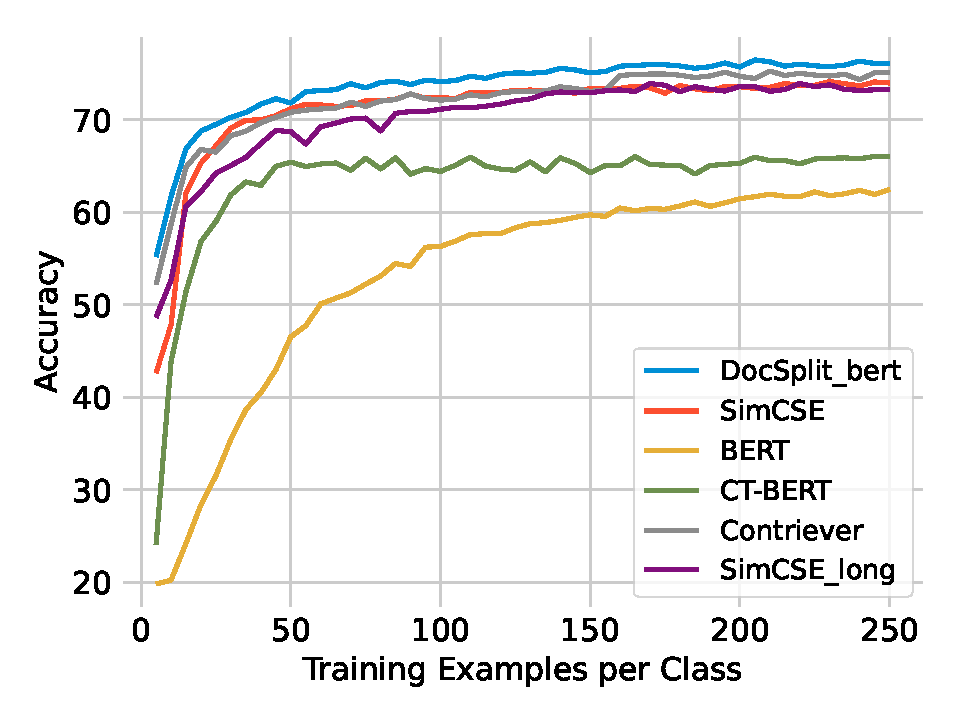
\includegraphics[width=0.8\linewidth]{fig/few_shot.pdf}
\caption{
    \ourbert~outperforms all other BERT-based models in a few-shot classification task on the 20News dataset.
    %\fixme{change x-axis to ``training examples per class''; change $\our$ to \ourbert, you can export the figure in tex instead of pdf to get the latex support needed for the legend}
}
\label{few_shot}
\end{figure}

%\textbf{Results.} 
%Table~\ref{results} shows the results of few-shot text classification on these five datasets. 
%We can see that, under the same model structure, \our~(i.e.,~\our$_{\mathrm{bert}}$ and \our$_{\mathrm{long}}$) achieves $12.0\%$ and $24.3\%$ macro-F1 improvements compared to SimCSE and Longformer respectively. 
%Surprisingly, INSTRUCTOR achieves low performance on the NYT and BBCNews under few-shot settings.
%%and achieves 0.028+0.082+2.03+0.769. 
%These improvements are higher than standard text classification. 
%Besides, we also compare the performance of different baselines (using BERT as a backbone) and \our$_{\mathrm{bert}}$ with different numbers of training instances on 20News. 
%The results in Figure~\ref{few_shot} show the improvements from our method become larger as the number of training instances decreases indicating the importance of high-quality document embeddings for low-resource settings. 
%Furthermore, our method achieves the best results under different numbers of training instances.

\subsection{Experiment 3: Document Retrieval}
%We conduct document retrieval to evaluate the ability to learn the similarity score between two vectors~\cite{Guo2016ADR} of documents.
We follow the document retrieval experiment of the Long Range Arena (LRA) benchmark \citep{Tay2020LongRA},
which uses the ACL Anthology Network (AAN) dataset \cite{Radev2009TheAA}.
The goal of the task is to predict whether two papers have a citation link given only their embeddings, which is a common setup used in long-form document matching~\cite{Jiang2019SemanticTM,Yang2020Beyond5T}.
This reduces to a binary classification task and accuracy is the commonly reported performance measure.
Figure \ref{retrieval} shows the results.
\ourbert~ outperforms all other BERT-based models, and \ourlong~ outperforms all other models.
%Specifically, for all baselines, we use models to obtain document embeddings and finetune an MLP layer on two concatenated embeddings to predict if two documents have a citation link.

%\textbf{Results.} 
%\begin{table}
%    \centering
%   \small
\begin{tabular}{l|c}
\toprule
Model   & Retrieval\\

\midrule
BERT   &53.56  \\
CT-BERT     &54.23 \\
SimCSE   &54.78\\
SimCSE$_{\mathrm{long}}$ &55.23 \\
cpt-text                   \\
INSTRUCTOR                 \\
\our$_{\mathrm{bert}}$   &58.29  \\
\midrule
LongFormer  &56.89  \\
BigBird     &59.29 \\
\our$_{\mathrm{long}}$  &59.89  \\
\bottomrule
\end{tabular}
%   \caption{}
%   \vspace{-3mm}
%   \label{retrieval}
%\end{table}

\begin{figure}
\centering
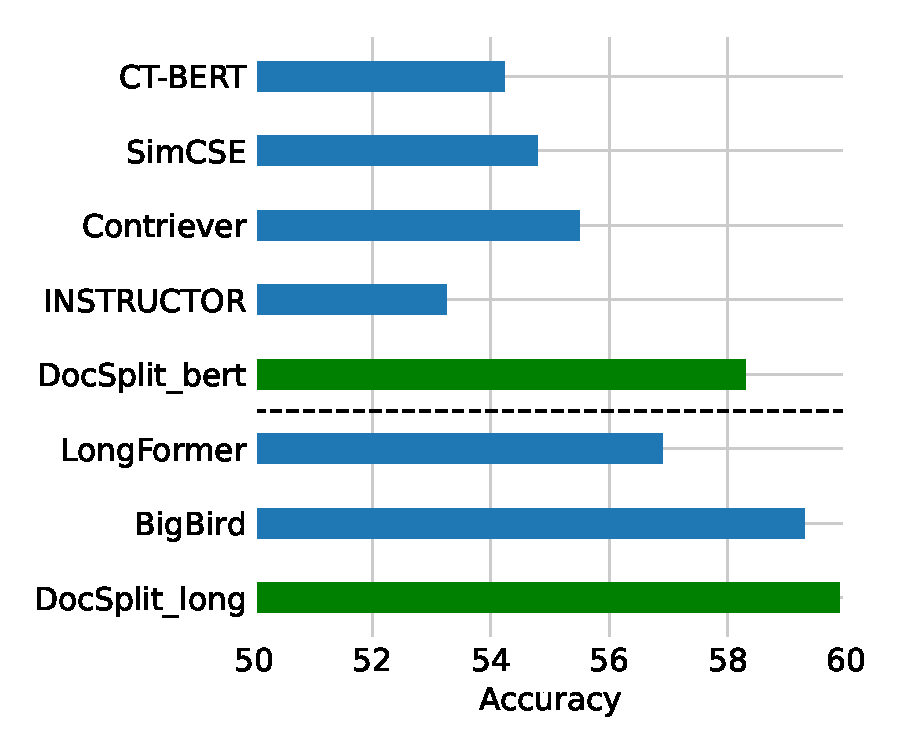
\includegraphics[width=0.8\linewidth]{fig/retrieval_fig.pdf}
\caption{In the standard LRA document retrieval task,
    \ourbert~ outperforms all other BERT-based models,
    and \ourlong~ outperforms all other models.}
\label{retrieval}
\end{figure}



%Table~\ref{retrieval} shows the results of the document retrieval experiment on AAN dataset.
%We can find that our method achieves the best results due to the effectiveness of our pretraining methods based on document splitting.

\section{Conclusion}
\label{sec:conclusion}
$\our$ is the first unsupervised pretraining method designed explicitly for large documents.
$\our$ can be used to pretrain any model architecture,
and we provide code to do so at
\begin{center}
    \url{https://blinded_for_review}
\end{center}
%$\our$ outperforms other pretraining methods for document classification, few shot learning, and document retrieval tasks.
The LongFormer-based \ourlong model provides SOTA performance on document classification, few-shot learning, and retrieval tasks.

\section*{Limitations}

%Our paper has three main limitations.
%\item Generative models cannot be trained using $\our$, but they can be trained using token masking.

We identify three limitations with our work.

\textbf{Limitation 1:}
We evaluate $\our$ using only three downstream tasks (classification, few-shot learning, and document retrieval),
but pretrained models are useful in many other tasks as well.
For example, the LongFormer \cite{Beltagy2020LongformerTL} is evaluated also on question answering and coreference resolution.
We did not run these experiments only due to a lack of computational resources,
and we hope that future work will evaluate the performance of $\our$ pretraining on other downstream tasks as well.
We note, however, that our $\our$ experiments in some ways are more extensive than other papers' experiments.
For example, the LongFormer paper does not include any document retrieval experiments, and we do.
Also, the Contriever model \citep{Izacard2021UnsupervisedDI} was specifically designed for pretraining models for the downstream retrieval experiment task and only evaluates on this downstream task.
We beat the Contriever model on this task and provide the classification and few-shot experiments in addition.

Much of the prior work on contrastive learning evaluates on a large number of tasks as well.
For example, INSTRUCTOR \cite{Su2022OneEA} is evaluated on 70 different downstream tasks.
None of these tasks, however, are applicable in our setting because these tasks include datasets with only small text and not large documents.

\textbf{Limitation 2:}
Our models are pretrained only on English wikipedia,
but other models are pretrained on significantly larger datasets.
For example, the LongFormer model was pretrained on English wikipedia and on the Books \citep{zhu2015aligning}, Real News \citep{zellers2019defending}, and Stories \citep{zellers2019defending} datasets.
We pretrained on this smaller dataset only due to our limited computational resources.
%For example, the INSTRUCTOR model was pretrained on a diverse range of 330 datatsets.
Results in scaling laws \citep{kaplan2020scaling} suggest that pretraining on more data would significantly improve our models' performance,
and so our results are reported results are likely underestimating the positive effects of $\our$ pretraining.

\textbf{Limitation 3:}
Our experiments do not evaluate how well $\our$ will work on extremely large (e.g.\ book length) documents.
Existing large document model architectures like LongFormer \cite{Beltagy2020LongformerTL} and BigBird \cite{Zaheer2020BigBT} are still not efficient enough to train models on these extremely large documents.
More work also needs to be done on generating suitable evaluation tasks in this extreme setting to understand $\our$ performance.

\section*{Ethics Statement}

Learning embeddings is a standard problem in natural language processing.
Our approach uses standard training datasets and training procedures.
There are therefore no direct ethical concerns with this research.
%We hope that our pretrained models and pretraining strategies will become widely used,
%but we have no control over whether
%As with all tools, however, the embeddings our model provides can be used for either good or evil.

Our total compute is relatively small and so we have a small environmental impact.
Pretraining \ourbert took 4 days on an Nvidia 2080 GPU with 11GB of RAM,
and pretraining \ourlong took 4 days with an Nvidia Quadro RTX 8000 with 48GB of RAM.
Other models use larger GPU clusters that require considerably more energy.
The finetuning procedures run in less than 1 day on the same systems.

%We do not anticipate any major ethical concerns; learning document embedding is a fundamental problem in natural language processing. Ethical considerations seem low-risk for the specific datasets studied here because they are all published.

%\section*{Acknowledgements}

% Entries for the entire Anthology, followed by custom entries
\bibliography{anthology,custom}
\bibliographystyle{acl_natbib}

\clearpage
\appendix
\section{Appendix}

\subsection{Training Details}
\label{app:details}
For text classification, the learning rate for fine-tuning is 3e-4; the batch size is 8; the maximum sequence length is 512 tokens. 
We fine-tune the last MLP layer on these five datasets and evaluate the classification performance with accuracy and macro-F1 scores.
For few-shot text classification, we sample 10 data instances per class for the FakeNewsCorpus dataset and the arXiv dataset and 5 data instances per class for the other three datasets. 
Other settings are the same as the standard text classification. 
Since there is randomness in sampling, we repeat every experiment 10 times and take the average value of metrics.

\subsection{Few-shot Learning}
\begin{table}
    \centering
    %\begin{tabular}{@{}lR{0.75in}R{0.75in}R{0.75in}R{0.75in}R{0.75in}R{0.75in}@{}}
\small
\begin{tabular}{l|cccccccccc}
\toprule
 Datasets   & \multicolumn{2}{c}{FakeNews}     & \multicolumn{2}{c}{20News}         &\multicolumn{2}{c}{arXiv}     &\multicolumn{2}{c}{NYT}        & \multicolumn{2}{c}{BBCNews} \\
 \cmidrule(l){1-1} 
\cmidrule(l){2-3} 
\cmidrule(l){4-5}
\cmidrule(l){6-7}
\cmidrule(l){8-9}
\cmidrule(l){10-11}
Metrics    & Acc & F1   & Acc & F1    & Acc & F1    & Acc & F1      & Acc & F1 \\

\midrule
\multicolumn{11}{c}{\textit{Few-shot Text Classification}}   \\
\midrule
BERT      &23.96  &23.73    &19.94  &18.71    &24.08  &10.14     &51.85  &43.90      &54.22  &52.73 \\
CT-BERT      &23.71  &23.06    &24.11  &23.53    &27.02  &13.53     &47.23  &36.83      &59.56  &58.95   \\
SimCSE      &25.04  &22.68    &42.63  &41.42    &32.61  &17.19     &86.51  &78.41      &83.56  &83.75    \\
SimCSE$_{\mathrm{long}}$ &26.39  &23.26    &48.65  &47.81    &23.42 &12.66  &85.36 &75.90   &84.44  &83.96 \\
Contriever     &24.17 &22.35  &54.27 &54.87  &33.19  &17.23     &84.73 & 77.62  &77.71 & 79.19        \\
INSTRUCTOR  &26.11 &23.97 & -- & -- &33.51 &17.12 &32.38 &27.60 &52.67 &48.78 \\
    \ourbert  &\textbf{27.79}  &\textbf{24.65}    &\textbf{55.79}  &\textbf{55.43}    &\textbf{35.79}  & \textbf{18.52}    &\textbf{90.52}  &\textbf{83.71}      &\textbf{86.86}  &\textbf{86.31}   \\
\midrule
LongFormer  &26.56  &25.12    &44.42  &42.41    &25.04  &13.36     &73.06  &54.87      &84.89  &85.47  \\
BigBird      &25.36  &23.28    &39.14  &39.06    &23.62 &10.18  &86.66 &78.96   &79.11  &76.63 \\
\ourlong  &\textbf{29.17}  &\textbf{27.13}    &\textbf{51.18}  &\textbf{50.96}    &\textbf{34.33}  &\textbf{18.80}   &\textbf{89.78}  &\textbf{82.88}      &\textbf{86.78}  &\textbf{86.66}  \\
\bottomrule
\end{tabular}

    \caption{Few-shot classification on five datasets. }
    \vspace{-3mm}
    \label{tab:few_shot}
\end{table}
Table~\ref{tab:few_shot} shows the results of few-shot text classification on these five datasets. 
We can see that, under the same model structure, \our~(i.e.,~\our$_{\mathrm{bert}}$ and \our$_{\mathrm{long}}$) achieves $12.0\%$ and $24.3\%$ macro-F1 improvements compared to SimCSE and Longformer respectively. 
Surprisingly, INSTRUCTOR achieves low performance on the NYT and BBCNews under few-shot settings.
These improvements are higher than standard text classification. 


% \subsection{Attention Weights}
% \label{app:attention}
% To explore the difference between \our~and other models, we analyze the attention weights of Transformers in different models on the NYT dataset (details in Appendix~\ref{app:attention}). The average weights of different kinds of words are shown in Figure~\ref{attentions}.  We can see that our model has more than $40\%$ higher attention weights on nouns compared to BERT and SimCSE.~\citet{martin-johnson-2015-efficient} shows nouns are more informative than other words in the document understanding. Hence, our pretraining method increases the attention weights of models on nouns which results in higher performance on long text classification. 

% \begin{figure}
% \centering
% 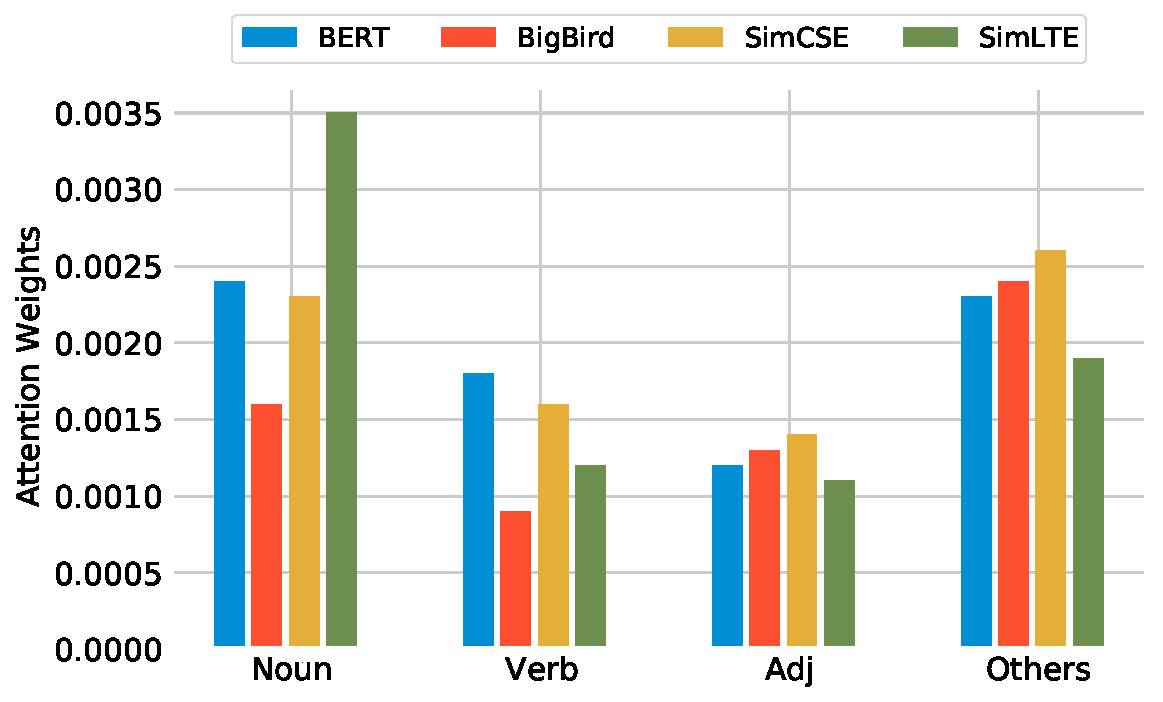
\includegraphics[width=0.8\linewidth]{fig/attentions.pdf}
% \caption{Attention weights from different models on the NYT dataset.}  
% \label{attentions}
% \end{figure}

% We compute the attention weights for Transformers as follows:
% (1) we first extract the attention weights between \texttt{[CLS]} token and all the other tokens;
% (2) we compute the averaged weights along different heads in multi-head attention;
% (3) the attention weights of the last layer in Transformers are used as the weights for words.
% Averaged values are computed for nouns, verbs, adjectives, and other words.

\end{document}